\section{Von der Black Box „Internet“ und dem Wesen der Kommunikation}
\subsection{Vom Brief zur E-Mail}
Wenn man sich in früheren Jahrhunderten etwas wichtiges und sehr privates mitzuteilen hatte, traf man sich persönlich, oder, wenn es die Distanz nicht erlaubte, engagierte man einen Vertrauenswürdigen Boten, der die Nachricht in Form eines Briefes mit Siegel (oder dergleichen) an die gewünschte Person überbrachte. Was den zweiten Fall betraf, so hatte man auch da nicht die volle Kontrolle. Man musste wohl oder übel auf den Boten vertrauen. Hinzu kommt, dass dem Boten ja auch unterwegs etwas hätte zustossen können oder der Bote gezielt abgefangen wurde. Es gab also schon immer Unsicherheiten, was die Übertragung von geheimen Nachrichten betrifft, sofern man es nicht komplett selbst in die Hand nahm. Mit der Entwicklung des Postwesens wie wir es heute kennen änderte sich vieles schlagartig. Briefe zu verschicken wurde bequem, einfach und bezahlbar. Jeder mit den nötigen Kleinutensilien konnte nun Briefe um die ganze Welt schicken, vorausgesetzt natürlich, man konnte schreiben. Wie sieht es mit privaten bzw. geheimen Briefen aus? Erfahrungen aus der Vergangenheit, wie zum Beispiel die Postkontrollen zu STASI-Zeiten, haben gezeigt, dass es je nach Regierungsform der einzelnen Länder unterschiedlich sicher war und noch heute ist, privates per Post mitzuteilen. Damals, in den 80er Jahren, wurde von der Abteilung M, welche für die Postkontrolle zuständig war, täglich bis zu 90 000 Briefe gelesen und/oder kontrolliert
\footnote{\url{http://www.briefmarkenverein-berliner-baer.de/vereinszeitung/241-1-stasi.htm}}. 
Der Briefverkehr wird aber auch heute noch rege genutzt für aller Hand oberflächlicher Kommunikation und nicht selten auch für Privates. In den 70er-Jahren kam schliesslich das Internet und mit dem Internet das grosse Zeitalter der E-Mail. Die E-Mail war zu Beginn die meistgenutzte und wichtigste Anwendung des Internets und schon 1971 brauchte der E-Mail-Verkehr mehr Datenvolumen als alle anderen Dienste zusammen
\footnote{\url{https://de.wikipedia.org/wiki/Internet\#Geschichte}}. 
Nachrichten konnten nun noch günstiger und vor allen Dingen schneller übermittelt werden. Es gab zudem keine topographischen Einschränkungen, wenn die Infrastruktur einmal vorhanden war. Mailverkehr übers Internet hat viele Vorteile, das kann man nicht bestreiten. Es hat aber auch eine sehr grosse Schwachstelle. Das Internet ist heute in seiner Komplexität so enorm und vielschichtig, dass es man als Laie kaum einschätzen kann, welchen Weg das verschickte Mail genau nimmt und welche Posten es dabei passiert. Hinzu kommt, dass das Internet eine Art Grauzone ist, was Recht und Ordnung betrifft und es in den undurchdringlichen Weiten viele technisch versierte Leute gibt, die vielleicht ganz bewusst die Kommunikation von Person XY anzapfen – ob nur zum Spass oder für Geld – es ist alles möglich.

\subsection{Der Webbrowser - Das Fenster zum Internet}
Ein weiterer Meilenstein in der Geschichte des Internets ist der Webbrowser. Mit der Einführung des ersten grafikfähigen Webbrwosers Mosaic im Jahre 1993 erhielt das Internet einen weiteren Aufwärtsschub
\footnote{\url{https://de.wikipedia.org/wiki/NCSA_Mosaic}}. 
Mit ihm war erstmals ein komfortables durchstöbern des World Wide Web möglich, ganz ähnlich, wie wir das heute mit bekannten Browsern wie dem Internet Explorer, Mozilla Firefox oder Google Chrome tun. Das Beispiel des Webbrowsers führen wir an dieser Stelle deshalb auf, weil es sehr gut zur Einführung in das nächste Kapitel dient.
Denn obwohl das Internet und das IT-Wesen allgemein immer komplexer und grösser werden, wird die oberflächliche Benutzung der Dienste immer einfacher. Kinder wissen oft schon ganz genau, wie und wo sie im Internat nach Informationen suchen müssen. Surfen wir im Internet, um nach irgendwelchen Angeboten oder Online-Artikeln zu suchen, sehen wir auf unserem Bildschirm lediglich ein Fenster, in dem wir die gewünschten Inhalte meist in strukturierter und visuell aufbereiter Form dargestellt bekommen. Es ist eine Schnittstelle in ein riesiges Netzwerk von enormer Komplexität, die den Laien wohl sehr schnell überfordern würde und trotzdem ist die Bedienung kinderleicht. Der Benutzer muss sich also nicht mehr um die technischen Details kümmern. Er muss sich nicht fragen, wie denn eigentlich die Informationen von A nach B kommen und wo sie gespeichert werden. Für diesen Sachverhalt gibt es einen Fachbegriff, man spricht von der sogenannten Black Box.

\subsection{Das Prinzip der Black Box}
Der Begriff Black Box hat einen wissenschaftlichen Hintergrund. Die englischsprachige Seite von Wikipedia gibt folgende Kurzdefinition des Begriffes an: 

\begin{quote} 
A black box is a device, object, or system whose inner workings are unknown; only the input, transfer, and output are known characteristics
\footnote{\url{https://en.wikipedia.org/wiki/Black_box_\%28disambiguation\%29}}.
\end{quote}

Auf Deutsch übersetzt heisst das so viel wie: ``Eine Black Box ist ein Gerät, Objekt oder System, dessen innere Funktionsweise unbekannt sind. Nur die Eingabe, der Transfer und die Ausgabe sind bekannt.''
Man gibt also etwas in die Black Box hinein und erwartet einen bestimmten Output. Was genau in der Black Box vorgeht, wie der Output entsteht, interessiert einen nicht. Es zählt nur das Ergebnis. Eine einfache Grafik soll das Prinzip verdeutlichen. 

\begin{figure}
\centering
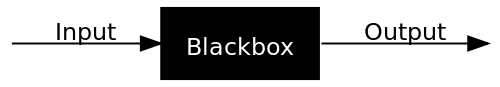
\includegraphics[scale=0.75]{images/BlackBox}
\caption{Black Box}
\end{figure}

Somit wären wir beim eigentlichen Thema dieser Arbeit angelangt. Die drei Anwendungsfälle

\begin{enumerate}
\item Surfen im Internet
\item Mailverkehr
\item Nutzung einer Cloud
\end{enumerate}

machen ebenfalls von der Black Box gebrauch. Surfen im Internet kann inzwischen schon ein Zehnjähriger, Trend nach unten steigend. Möchte man einen Mailaccount einrichten, kann man dies gratis und innert fünf Minuten erledigen. Der Anbieter führt einem dabei Schritt für Schritt durch die Einrichtung des Accounts und hält einem während der ganzen Zeit die Hand. Was die Cloud angeht, so ist deren Nutzung für den Normalverbraucher noch nicht so selbstverständlich, wie surfen und E-Mail. Doch auch hier ist ein Trend zur vermehrten Verbreitung und Nutzung erkennbar. Im technischen Umfeld und in Unternehmen hat sich die Cloud aber schon längst durchgesetzt. Auch hier wird man meist mit technischen Problemen verschont. Der Anbieter kümmert sich um die technischen Dinge, während man selbst nur das simple Programm bedient.
\\
\\
Es macht durchaus Sinn, dass man Dienste bewusst auslagert und konzentriert. Es kann schliesslich nicht jeder Mensch dieser Welt IT-Spezialist sein. Dafür gibt es schlicht zu viele Menschen, zu wenig Zeit und Ressourcen und zu schnell wachsender Fortschritt. Warum sollte man dann die technischen Fragen nicht denen überlassen, die sich in diesem Gebiet spezialisiert haben? Eine mögliche Antwort darauf gaben uns die letzten paar Monate, seit Edward Snowden, ehemaliger Mitarbeiter bei der NSA, mit höchst brisanten Dokumenten an die Öffentlichkeit gegangen ist.Aus den Dokumenten geht hervor, dass gewisse Geheimdienste, allen voran die amerikanische NSA, (engl. National Security Agency) massiv Daten aus dem Internet angreift. Dies betrifft den Mailverkehr, Daten in der Cloud und Daten bezüglich dem Surfverhalten der jeweiligen Nutzer. Ähnlich wie früher beim Boten, legt man auch heute die Daten in die Hände von Dritten, meist grosse, internationale Unternehmen, welche diese dann verarbeiten. In die Einzelheiten des Verarbeitungsprozess hat man dabei keinen Einblick, es ist eine Black Box. Es war also bis heute alles eine Frage des Vertrauens und wird es vielleicht auch in Zukunft sein.
\\
\\
Die Enthüllungen Snowdens und die dadurch entstandenen, hitzigen Diskussion zeigen eines ganz klar auf: Es braucht dringend ein neues Bewusstsein, was das Internet, dessen Möglichkeiten und Gefahren und die Privatsphäre betrifft. Die Frage des Datenschutzes ist einmal mehr in aller Munde und das zu recht. Wenn  Der gläserne Mensch, ein Mensch ohne Privatsphäre und Geheimnisse, scheint in greifbarer Nähe und ist er einmal Realität, lässt er sich nur schwer wieder verbannen
\footnote{\url{https://de.wikipedia.org/wiki/Gl\%C3\%A4serner_Mensch_\%28Datenschutz\%29}}.
\\
\\
Die Redewendung „Vertrauen ist gut, Kontrolle ist besser!“, die ironischerweise dem russischen Politiker Lenin zugeordnet wird
\footnote{\url{https://de.wikipedia.org/wiki/Vertrauen_ist_gut,_Kontrolle_ist_besser!}}, 
trifft die Haltung recht gut, die wir teilen. Der Nutzer sollte mehr Kontrolle darüber haben, was mit seinen Daten passiert oder zumindest genau darüber Bescheid wissen. Es gibt dazu unterschiedliche Ansätze und sehr viele Möglichkeiten, diese Kontrolle (zurück-)zuerlangen. Unser Ziel ist es dabei, die Ansätze und Möglichkeiten zu finden, die dem Laien möglichst wenig technisches Know-How abverlangen, einfach umzusetzen sind und trotzdem die grösstmögliche Kontrolle bieten.
%Quellen:
%https://de.wikipedia.org/wiki/Post
%https://de.wikipedia.org/wiki/Geschichte_der_Post
%https://de.wikipedia.org/wiki/Ministerium_f\%C3\%BCr_Staatssicherheit
%http://www.briefmarkenverein-berliner-baer.de/vereinszeitung/241-1-stasi.htm
%https://de.wikipedia.org/wiki/Internet\#Geschichte
%https://de.wikipedia.org/wiki/NCSA_Mosaic
%https://de.wikipedia.org/wiki/Gl\%C3\%A4serner_Mensch_\%28Datenschutz\%29
%http://de.cyclopaedia.net/wiki/Vertrauen-ist-gut,-Kontrolle-ist-besser-1
%https://de.wikipedia.org/wiki/Vertrauen_ist_gut,_Kontrolle_ist_besser!

%Bilder:
%https://upload.wikimedia.org/wikipedia/commons/thumb/f/f6/Blackbox.svg/500px-Blackbox.svg.png
